%%%%%%%%%%%%%%%%%%%%%%%%%%%%%%%%
\section{The Electronics, Chimneys and DAQ}
\label{sec:detectors-fd-alt-elec}

The large number of charge readout channels, needed for the 20--50~kt
LAr detectors developed in the LAGUNA-LBNO design study with channel
count in the range of 500,000 to 1,000,000, naturally called during
the last years for R\&D efforts in view of the development of large
scale charge readout solutions. These are characterized by
high-integration levels, significant cost reduction and aims to
performance improvement.

The related R\&D activities (ongoing since 2006) have focused on two main axes:
\begin {itemize} 
\item{Development of cold front-end ASIC electronics}
\item{Development of low cost, largely scalable, data 
acquisition system based on modern telecommunication technologies.}
\end{itemize}

Both efforts aim at improving the effectiveness and the integration
level of the complete readout chain and cost reductions for the large
number of channels to be implemented in the detector. One of the goals
of the WA105 6$\times$6$\times$6~m$^3$ demonstrator including 7680
charge readout channels, is to establish this large scale readout
system developed in the LAGUNA-LBNO design study. A detailed
description of the charge readout electronics including the cold
front-end ASICs and the data acquisition system, and the related
references, is available in the WA105 Technical Design Report and in
the Status report document submitted to the CERN SPSC committee in
March 2015\cite{WA105_TDR},\cite{WA105_SREP}.

The design of the electronics was driven by costs reduction and by its
particular use for the dual-phase readout, which allows releasing
some requirements. In the dual-phase design the ionization electrons
are collected by a segmented anode in the gas phase (GAr) at the top
of the detector, the Charge Readout Plane (CRP). The anode sandwich
incorporates the Large Electron Multipliers (LEM) which amplify the
ionization charges by at least a factor 20 with avalanches occurring
in the pure GAr within the strong electric field regions of the
LEM. The LEM gain is tunable from the minimal requirement of 20 up to
200, by adjusting the LEM voltage. The electrons then reach the strips
of the segmented anode Printed Circuit Boards where they are equally
shared among two perpendicular collection views. The front-end
amplifier connected to the anode, given the capacitance of the anode
strips, would have at unitary LEM gain a signal to noise ratio of
14. Considering a minimal LEM gain of 20 the amplifier provides an
overall S/N ratio of 140. The signal to noise ratio is boosted by the
LEM gain and this releases the requirements on the preamplifier
noise. The front-end amplifiers are implemented as cryogenic CMOS
ASIC. Given the fact that the anode is at the top of the detector the
front-end can be connected with short (50~cm) cables and kept at cold
but in specific volumes (chimneys) completely separated from the one
containing the pure LAr and gas argon. The front-end electronics is
cryogenic and located at short distance from the detector, both
aspects concurring to the noise reduction, but it is completely
accessible from outside and it can be replaced at any time without
contaminating the LAr inside the cryostat. Flat cables (2~m long)
inside the chimneys connect then the front-end cards to the
digitization electronics which is outside the cryostat, hosted in
microTCA crates at the exit of the chimneys. This solution based on
accessible cryogenic front-end and external digital electronics
provides risks mitigation and large flexibility. The digitization
units in the micro-TCA crates are synchronized with the White Rabbit
time distribution standard which was originally designed designed to
achieve sub-ns accuracy. This built-in accuracy is much better than
the one which one would need in order to align the 400~ns samples of
the charge readout and it is not a critical aspect of the system
design. White Rabbit was adopted on the basis of practical integration
aspects and cost reduction. Its very good timing accuracy comes as an
extra bonus, White Rabbit is also used as an independent network for
the trigger distribution. The light readout digitization electronics
is also implemented in micro-TCA and provides triggers from the
photomultipliers which are distributed to the DAQ via the White Rabbit
network. Commercial high bandwidth and high computing power back-end
cards are used for event building and are coupled to a farm for online
processing which is implemented for event filtering, data
reconstruction, calibrations and data quality assessment. Details on
the system are given in the following.


\subsection{Front-end cryogenic amplifiers}
In the framework of the R\&D related to LAGUNA-LBNO, since 2006,
several generations of prototypes of ASIC 0.35 microns CMOS
multi-channel preamplifier chips operating at cryogenic temperatures,
have been developed. On one hand this implementation provides the
advantage of shortening the length of the cables and the associated
capacitance for the connection to the detector (in the dual-phase
design implemented in WA105 these cables are just 50~cm long). On the
other hand it allows reaching an optimal amplifier S/N ratio at a
temperature around 110~K, which can be easily achieved in the GAr at
the top of the cryostat. The other feature of this R\&D program is
that the cryogenic front-end electronics, although at very short
distance from the detectors in the CRP is perfectly accessible at any
time without opening the cryostat. This is achieved by implementing
the front-end cards at the bottom of the ad-hoc designed chimneys
which have two feedthroughs (a warm and a cold feedthrough). The cold
feedthrough isolates the cards from the inner volume of the
vessel. The chimneys are filled with inert gas and have a cooling
system to keep the electronics at the optimal temperature.

The first ASIC versions were generally designed for the readout of
charges from collection and induction wire planes, dealing also with
bipolar signals. Since 2012 some specific versions for the
dual-phase were produced in order to match the dynamic range of the
signals coming from the two collection views of the anode PCB after
LEM amplification. In this scheme, each collection view is
instrumented with strips of 3.125~mm pitch and 3~m length (150~pF/m
capacitance), as foreseen in the WA105 experiment. With a 3.125~mm
strips pitch, simulations of electromagnetic showers predict that a
single channel may collect up to 40~MIP. The design of the
dual-phase cryogenic ASIC is currently based on a LEM minimal gain
of 20 which corresponds to 1200~fC for this maximal signal of 40~MIP.

There are actually two produced versions of the dual-phase ASIC
chips for WA105, both with 16 readout channels. A first ASIC version
has a constant gain in the region 0--40~MIP. The second version is
characterized by a double-slope gain. This solution optimizes the
resolution while preserving a large dynamic range. It is characterized
by a high gain region extending up to 10~MIP signals. After 10~MIP the
gain is reduced by a factor 3 in order to overall match a dynamic
range of 40~MIP. This solution provides the best resolution in the
MIP region (dE/dx measurements ) without limiting the dynamic range
for showers, which can still reach up to 40~MIP (see
Figure~\ref{fig:FE_ASIC1}). This double-slope regime has been
optimized on the basis of simulations of hadronic and electromagnetic
showers. Both ASIC versions, compatible with the LEM signals dynamics,
are realized in the CMOS 0.35~$\mu$m technology, have 16 channels,
18~mW/channel thermal dissipation or less, about 1300 electrons ENC at
250~pF input detector capacitance and operate with this best S/N ratio
figure around a temperature of 110~K.
\begin{cdrfigure}[Dual-phase cryogenic ASIC amplifiers]{FE_ASIC1}
{Front-end 16 channels cryogenic ASIC amplifier with the double-slope gain implementation}
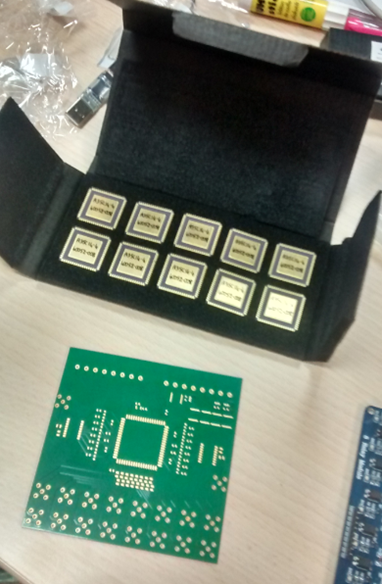
\includegraphics[width=.3\linewidth]{FE_ASIC2}
\end{cdrfigure}

The implementation of the double-slope gain regime is obtained by
replacing the feedback integration capacitor of the OPAMP with a MOS
capacitance which changes its value above a certain threshold
voltage. This effect is also present during the discharge phase and it
can be corrected with the inclusion in the feedback loop of an
additional branch with a diode and a resistor designed to keep the RC
value about constant during discharge. This branch can be
selected/deselected with an internal switch for all the channels in
the ASIC (see Figure~\ref{fig:FE_doubleslope}).
\begin{cdrfigure}[Double-slope ASIC response]{FE_doubleslope}
{Response of the double-slope ASIC amplifier to progressively larger 
pulses with and without the diode/resistor feedback branch}
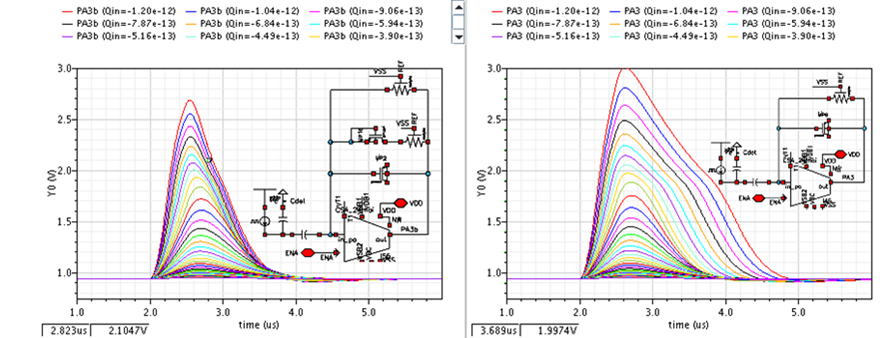
\includegraphics[width=\linewidth]{FE_doubleslope}
\end{cdrfigure}

In the design under implementation in WA105 and proposed for DUNE
there are 640 channels per chimney. The 40 ASIC amplifiers needed for
the readout of each group of 640 channels will be arranged on 10 pairs
of FE cards plugged in the feedthrough at the bottom of each chimney.
Each front-end card hosts two ASIC chips and a few discrete
components. Particular care has been taken in testing several options
(Gas Discharge Tubes, Metal Oxyde Varistors, double diodes) for the
surge arrestor components which have to protect the ASICs from
occasional sparks occurring in the CRP.  This study was aiming at
maximizing the protection efficiency, testing the components
durability for a very high number of sparks and minimizing the input
capacitance seen by the pre-amplifiers. Double-diodes have been
selected as the best solution given their performance and
capacitance. The total dissipation of the front-end electronics will
be of about 11.5~W per chimney. This heat source is minor with respect
to the heat conduction from the flat cables going to the digitization
electronics and from the walls of the chimney. The front-end cards are
kept at low temperature by a cooling system installed at the bottom of
chimney and compensating this overall heat flow. The front-end
electronics is coupled to the DAQ system, described in the following,
based on 12 bits ADCs, well matching the needed dynamic range.

Figure~\ref{fig:chimneys_scheme} shows the 3D model of the signal
feedthrough chimneys hosting the cryogenic ASIC amplifiers.
\begin{cdrfigure}[3D model of the signal feedthrough chimneys]
{chimneys_scheme}{3D model of the signal feedthrough chimneys}
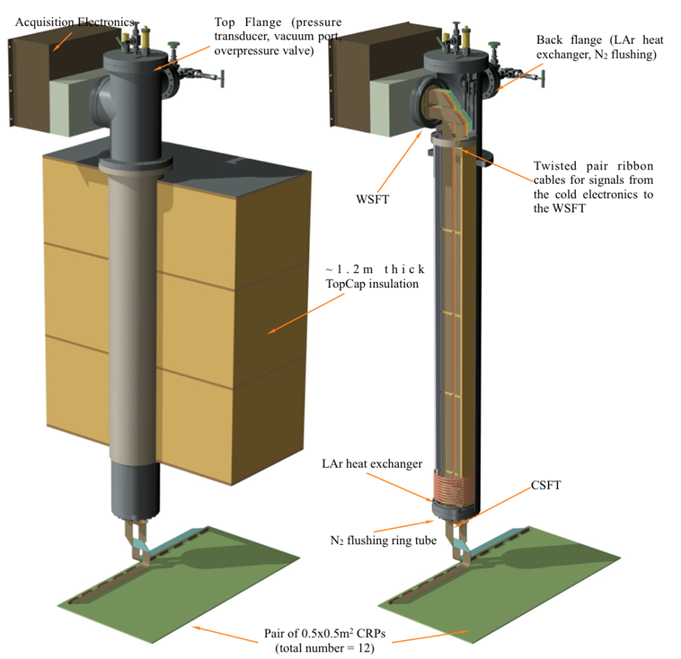
\includegraphics[width=.5\linewidth]{chimneys_scheme}
\end{cdrfigure}
A signal FT chimney prototype for 320 channels built for the
3$\times$1$\times$1~m$^3$ WA105 prototype is shown in
Figure~\ref{fig:chimneys_proto}.
\begin{cdrfigure}[Prototype of the signal feedthrough chimneys]
{chimneys_proto}{Prototype of the signal feedthrough chimney built 
for the WA015 3$\times$3$\times$1~m$^3$ prototype}
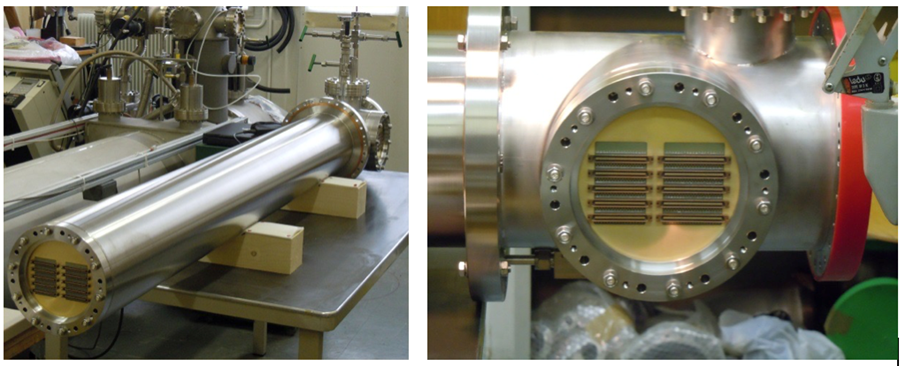
\includegraphics[width=\linewidth]{chimneys_proto}
\end{cdrfigure}
Pairs of cryogenic electronics FE cards are mounted at the end of
sliding G10 blades which can be extracted from the top of the
chimney. The blades, which are also carrying the flat cables for the
connections, slide on some guides mounted inside the chimney. By
moving the blades the FE cards can be plugged/unplugged on the
connectors present on the top side of the cold feedthrough located at
the bottom of the chimney. This feedthrough completely isolates the
chimney from the LAr vessel and has on its bottom side other
connectors for the 50~cm flat cables which are used to connect the
signals from the CRP.


\subsection{Digital electronics and DAQ global architecture}

The global DAQ system which is proposed for the dual-phase DUNE
detector design is based on 2 industrial standards:
\begin{itemize}
\item MicroTCA ($\mu$TCA) standard for the distributed data network \cite{mTCA-standard}
\item White Rabbit (WR) standard for the distributed clock network \cite{WR-standard}
\end{itemize}

The global DAQ scheme foresees that electrical signals transit from
the front-end electronics ASICs through the signal chimneys. The
signals are then collected by digitization boards in the $\mu$TCA
standard which offers data connections through a 10GbE network
(L1). Each $\mu$TCA crate (shelf) is connected through a 10GbE up-link
to the next level (L2). The L2 directly connects the micro-TCA crates
to high performance, FPGA based, back-end processing boards for event
building. A lossless transmission scheme is foreseen down to the
back-end processing board which applies all filtering algorithms and
the event building. The Huffman lossless algorithm is of easy
implementation and provides a typical factor 10 compression on liquid
argon events.

Recorded data are sent to a local storage level where Object Storage
Servers (OSS) and MetaData Servers (MDS) are connected with the event
building workstations via a 10/40GbE network (Ethernet or
InfiniBand). In parallel, a high stability common clock and time
synchronization signals are distributed to L1 digitization cards,
using the White Rabbit standard, through a dedicated, deterministic
network, together with the trigger time-stamp signals. The trigger
signals can be generated by the PMTs readout electronics or by
additional sources, as the beam trigger counters in the case of the
WA105 operation on the charged particle beam. The clock is derived
from a Master Clock generator connected to the White Rabbit
Grand-Master switch. This DAQ scheme is being implemented on the WA105
demonstrator at CERN, additional details may be found in\cite{WA105_TDR}.

\subsection{MicroTCA standard and applications}
The $\mu$TCA standard offers a very compact and easily scalable
architecture to handle a large number of channels at low cost. The
$\mu$TCA or related standards --- such as ATCA or xTCA --- are now well
known in the HEP community and have been integrated in various designs
at CERN (LHC upgrades), DESY, etc.  $\mu$TCA fulfills requirements of
the telecommunication industry and offers the possibility to
interconnect distributed applications while offering a standard,
compact and robust form factor with simplified power supply
management, cooling and internal clocks distribution. The backplane in
a $\mu$TCA crate (so-called $\mu$TCA shelf) is based on high speed
serial links arranged in various possible topology to support a large
variety of protocols: Ethernet 1GbE or 10GbE, PCI Express, SRIO
etc. The proposal is to use Ethernet-based solutions, both for data
and clock distribution, through the $\mu$TCA backplanes. This choice
obviously optimizes the connections between the various nodes of the
system. Constraints on the data transfer bandwidth impose to employ
the 10GbE protocol, which is defined in the $\mu$TCA standard. For the
clock distribution, dedicated lanes must be defined by the user. The
standard offers so-called clock lanes which distribute all boards
within the crate and which may be used for any particular signal.

The signals digitization boards plugged into a $\mu$TCA shelf are
called Advanced Mezzanine Card (AMC)\cite{picmg-2006}. Each AMC board
is connected to one or two MicroTCA Carrier Hub (MCH) boards through
the backplane serial links. The MCH provides a central switch function
allowing each AMC to communicate with each other or towards external
systems, through an up-link access. The MCH manages both the 10GbE
uplink and the WR bi-directional clock distribution.
Figure~\ref{fig:mTCA-features} provides a sketch of the backplane
layout and its implementation in one retained shelf reference.
\begin{cdrfigure}[MicroTCA crate organization]{mTCA-features}
{\small Left: global microTCA crate organization. AMC cards 
(providing basic ADC functions) are connected to the crate 
controller or MCH which up-links the external systems. A dedicated 
AMC for the clock receives dedicated signals (masterclock, trigger 
signals) from the timing distribution system and transcript them onto 
the backplane. Right: backplane layout of the Schroff 11850-015 reference.}
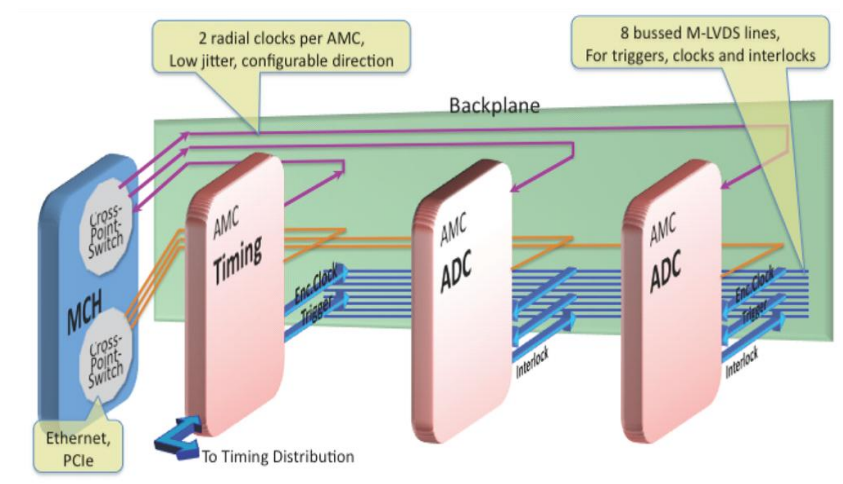
\includegraphics[width=.5\linewidth]{fig-mTCA-sketch.png}\hfill
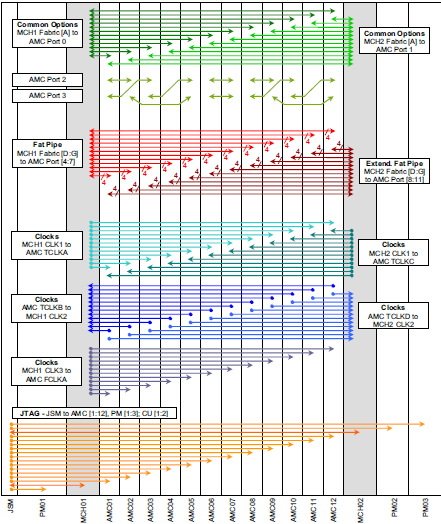
\includegraphics[width=.4\linewidth]{fig-mTCA-bckpln.png}
\end{cdrfigure}

The production version designed for the WA105 DAQ is based on the
$\mu$TCA.1 standard, with connections to the detector signals from the
front side only of the MCAs. These connections are made with VHDCI
cables in order to minimize the number of cables. One $\mu$TCA shelf
is connected to each signal chimney, reading out 640 channels.  The
shelf hosts 10 AMC digitization boards with 64 channels per board.

%To increase the channels density one may profit of a different $\mu$TCA standard: $\mu$TCA.4. This standard offers the possibility to connect the AMCs hosted in a crate from both the front and rear sides (Figure~\ref{fig:schroff-mTCA-4}). The front card, still called AMC, is connected to the backplane of the shelf, while the read card, so-called $\mu$RTM (Rear Transition Module) is only connected to the AMC. This standard allows to double the number of connections per slot, at the cost of a slightly asymmetric design for the 2 boards. 

Many references exist on the market for these various types of off-the-shelf products:
11850-015 8U from Schroff for $\mu$TCA.1 standard, NATIVE-R9 from NAT
for $\mu$TCA.4 standard. The cost of those items is quickly
decreasing, profiting from the fast developments of the internet
providers. They have redundant power supplies, redundant MCHs and
offer different segmentation to connect the AMC boards.


%\begin{cdrfigure}[General organization of AMC]{schroff-mTCA-4}{\small Left: general organization of AMC and $\mu$RTM boards in $\mu$TCA.4 standard. %Right: picture comparing $\mu$TCA.4 boards and a VME board.}
%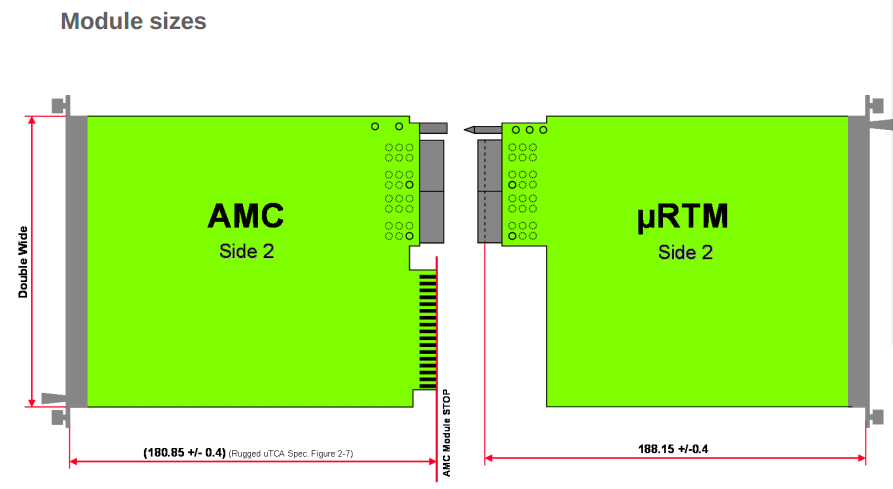
\includegraphics[width=.5\linewidth]{fig-mTCA-4-1.png} \hfill
%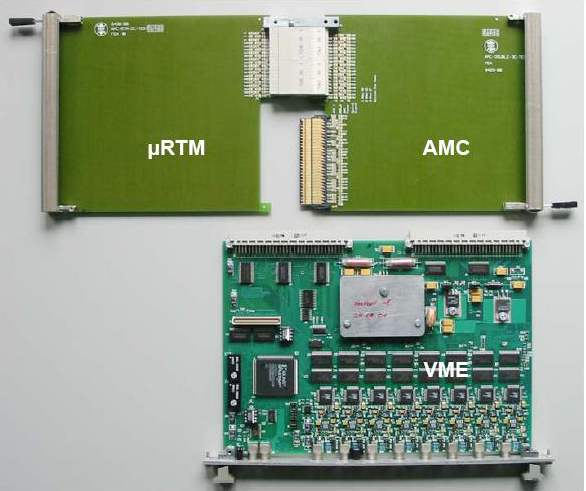
\includegraphics[width=.4\linewidth]{fig-mTCA-4-2.png}
%\end{cdrfigure}

The advantage of this architecture is to limit the DAQ electronics
developments to the AMC boards only. The AMC will basically provide
the functionalities for the digitization, data formatting and
compression, event time-stamping and data transfer through the
backplane. For WA105, the AMC is a double-size module (also compatible
with $\mu$TCA.4 standard) with a single input connector and a 10GbE
link to the backplane. The input stage performs the 64 channels
digitization through eight 8-channel, 14-bit ADC chips readout at a
2.5~MHz frequency. The ADC readout sequence is controlled by 2 FPGAs
which make the data available on a double port memory. Readout of the
data is performed continuously and they are stored in a local
buffer. The recorded samples, corresponding to a drift window, are
selected in coincidence with the received trigger. When a trigger
occurs, the samples written in the memory, can be treated with
compression algorithms (such as Huffman or RLE) or zero-suppression
(if required) and transmitted over the network until the end of the
drift window which closes the event. These operations are managed by a
third FPGA, which sends the data on the backplane.  This readout
scheme and hardware implementation have been validated for WA105 on a
Stratix 4 prototype board, shown in Fig.~\ref{fig:AMC-bloc-diag}.
\begin{cdrfigure}[Charge readout AMC board prototype]{AMC-bloc-diag}
{\small Prototype of AMC board, using $\mu$TCA.1 standard, and hosting 
64 ADC channels on a mezzanine board. This prototype is used as a validation 
of the full and final ADC chain in WA105.}
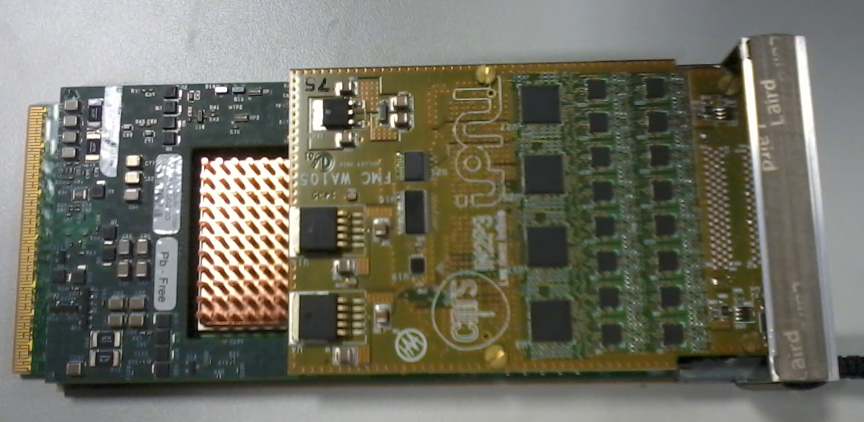
\includegraphics[width=.5\linewidth]{fig-s4am.png}
\end{cdrfigure}

\subsection{Back-end and event builder}


A network hierarchical structure is implemented where all crates are
interconnected to a dedicated back-end FPGA processing board (such as
S5-PCIe-HQ, Figure~\ref{fig:Bittware-board}). 
\begin{cdrfigure}[FPGA processing board]{Bittware-board}
{\small FPGA processing board based on Stratix V from Altera. The board 
features a dual QSFP+ cages for 40GigE or 10GigE links, 16 GBytes DDR3 SDRAM, 
72 MBytes QDRII/II+, two SATA connectors and is programmable via OpenCL.}
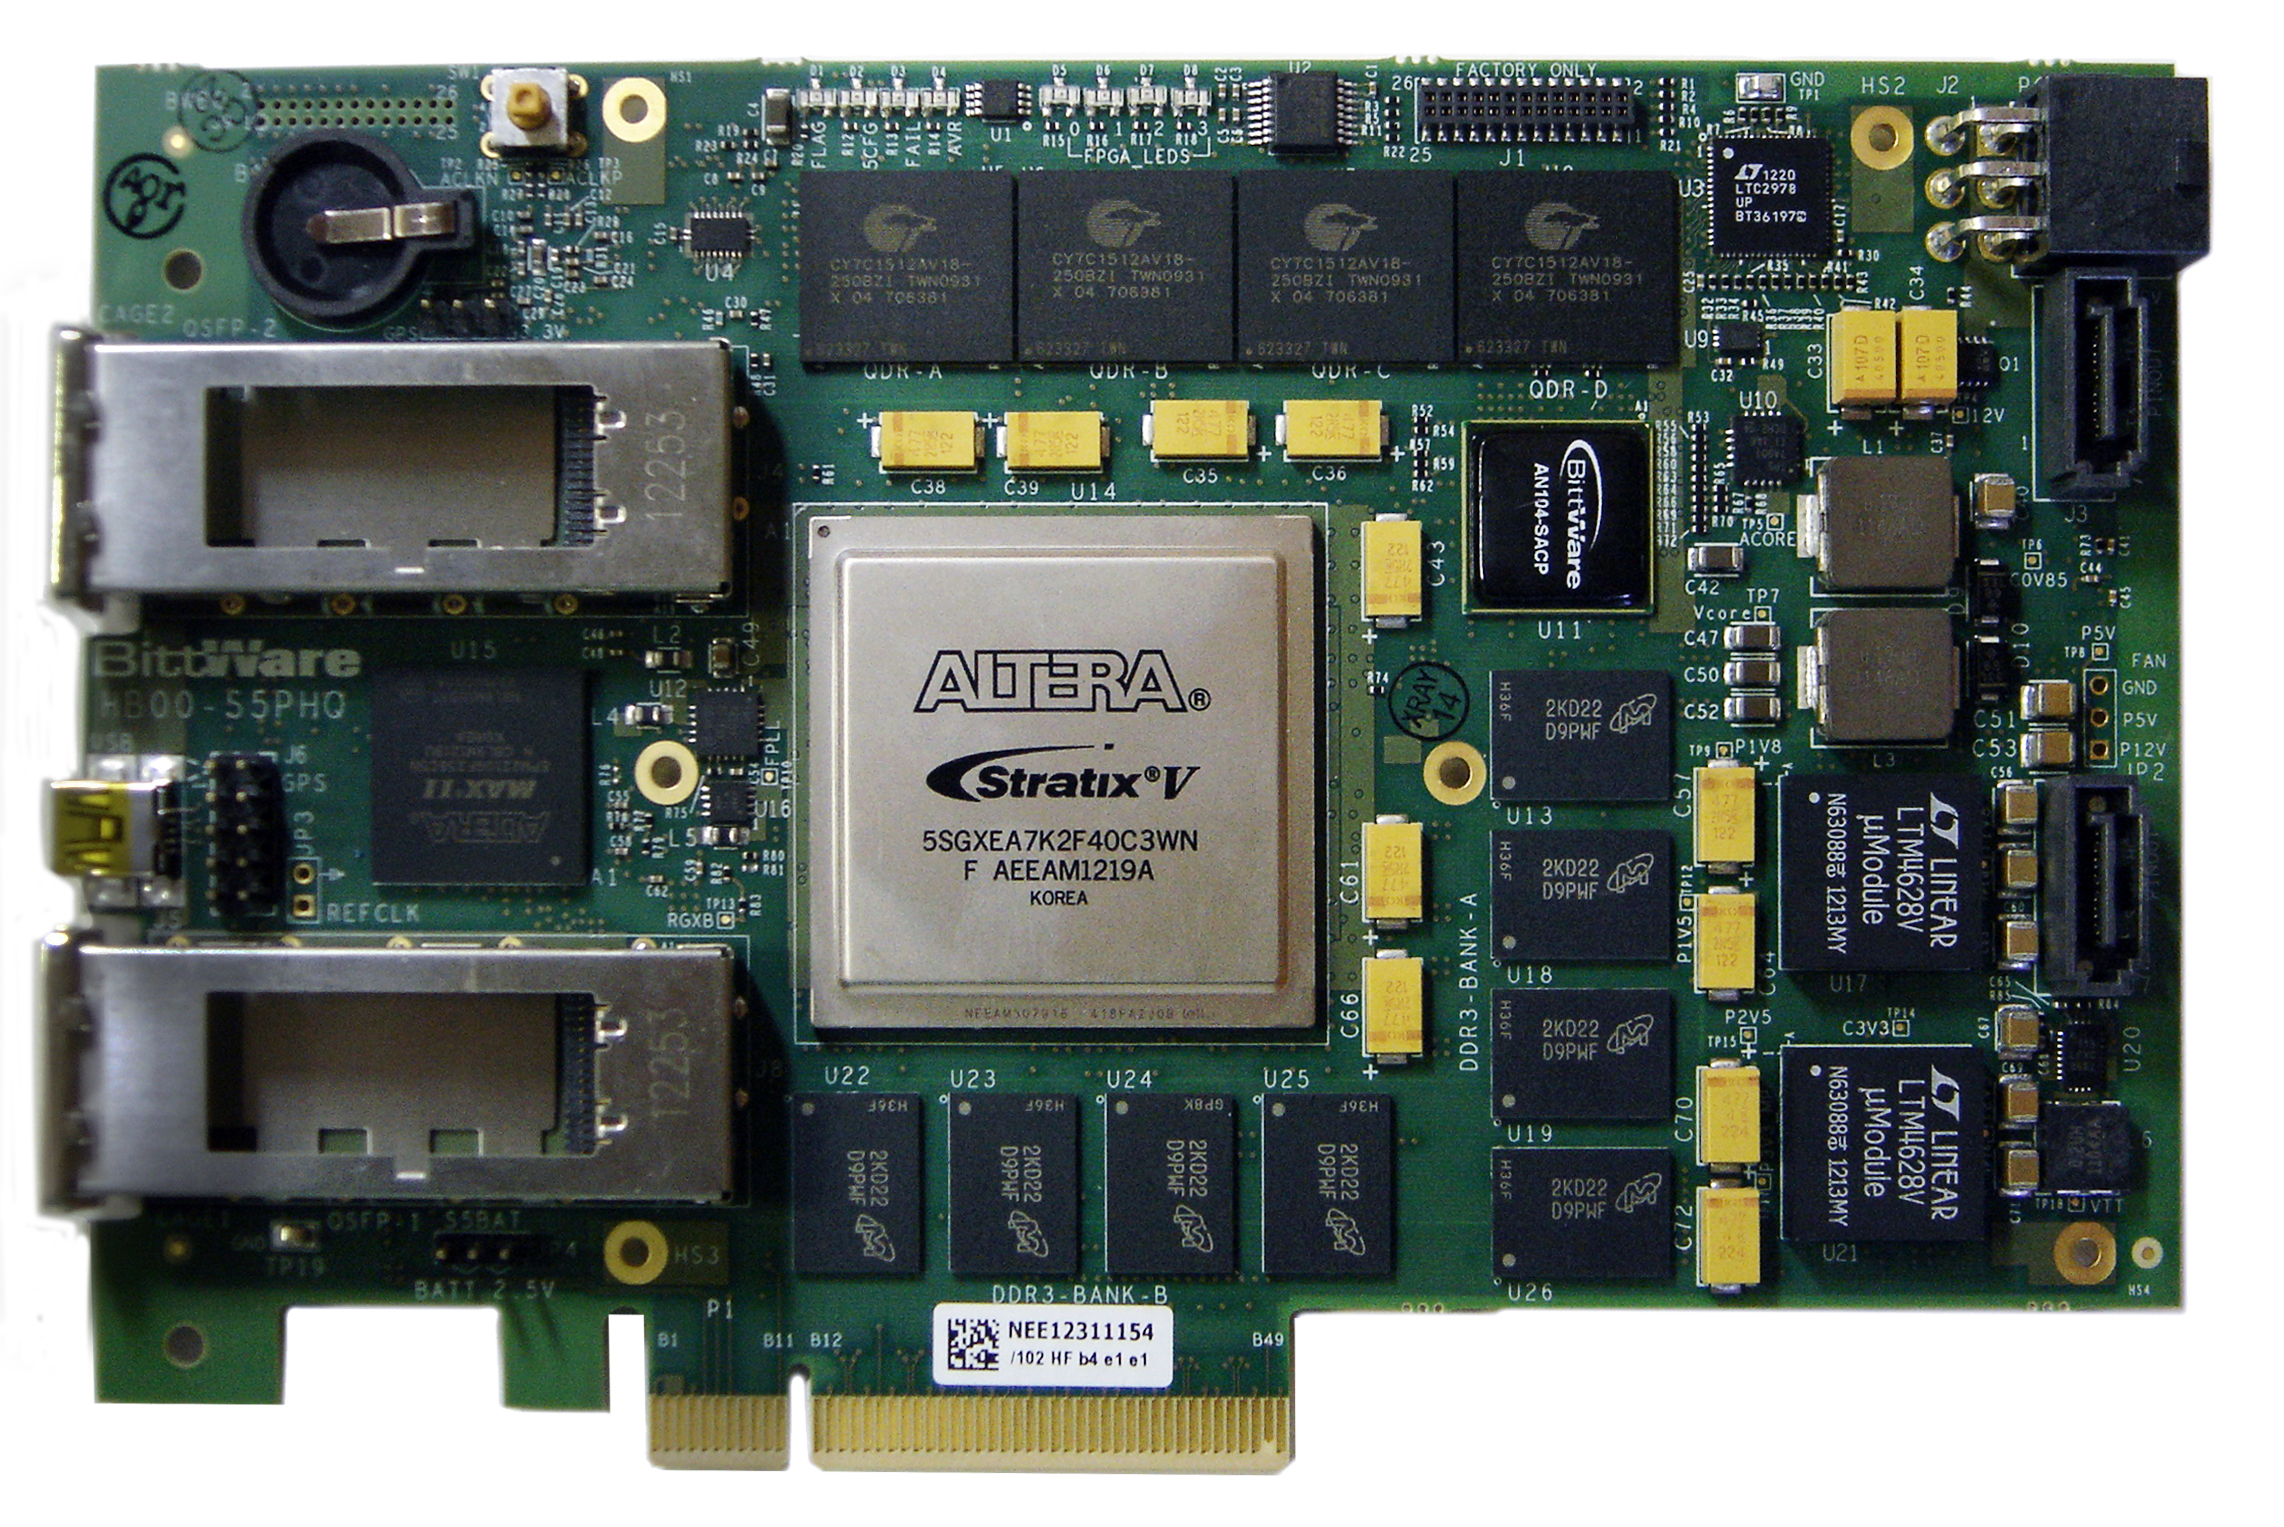
\includegraphics[width=.4\linewidth]{fig-bittware.jpg}
\end{cdrfigure}
This kind of board is used for massive processing in many fields
(medical imaging, stock exchange market etc) which require parallel
processing with reduced power consumption (only 10\% of the power
dissipated by an equivalent CPU for a comparable number of
operations). This particular board has two QSFP+ cages to bring the
data directly to the FPGA for lowest possible latency. Up-to 8x10GbE
links w/o data loss are available per board.  The board performs
further data processing, filtering and transmission to the highest
level for storage. This type of board is widely used and the present
generation, based on the Altera Stratix V, will evolve to the Aria X
and the Stratix X. This version will be probably available at the time
of the construction of the DAQ system. Programming of the back-end
processing board is achievable through the OpenCL software suite where
a kernel code allows, on top of a host code, to program directly in
high level language the FPGA without a classical VHDL synthesis
chain. OpenCL applications are transparent to the hardware used for
procesing (FPGAs, CPUs, GPUs). This highly flexible feature is fully
adapted to the requirements of the large DAQ systems, where conditions
of filtering, event building etc may evolve with time.
 
\subsection{Timing distribution system and White Rabbit standard}

The idea for the clock distribution is to use a parallel, independent
network from a GPS disciplined Master Clock down to each $\mu$TCA
shelf, through specific switches. Technically the WR standard is based
on a combination of Synchronous Ethernet (Sync-E) and Precision Time
Protocol (PTP, IEEE1588), where the Ethernet clock is generated by a
GPS disciplined clock. At the level of each shelf, this high accuracy
clock is made available to each AMC board through dedicated lines of
the backplane. As discussed before, the $\mu$TCA standard foresees
special lanes for clock transmission. The trigger signals
(time-stamps) are encoded and sent through this dedicated WR network
which has enough bandwidth for this transmission without interfering
with the PTP synchronization signals. The requirements on the
synchronization for the charge readout are quite loose since the
typical readout frequency is of the order of a few MHz. The
requirements for the PMT readout on the contrary are more
stringent. The goal is to provide a nanosecond synchronization at the
level of all L1 elements. This goal is typically achievable with the
White Rabbit (WR) standard\cite{WR-standard}.

The WR provides an extension to Ethernet network with Gigabit data
transfers and accurate synchronization among its different
elements. It provides a common clock for physical layer in the entire
network, allowing sub-nanosecond synchronization accuracy and 20~ps
jitter time. The WR network is designed to host up to thousands of
nodes and to support distance ranges of 10~km using fiber cables. It
ensures that all the Ethernet frames sent are delivered at least after
a fixed delay (controlled latency). The order of the frames should be
preserved.  A typical application scheme is displayed in
(Figure~\ref{fig:WR_elements}).
\begin{cdrfigure}[White Rabbit network organization]{WR_elements}
{\small Left: general organization of a typical WR network. Right: standalone WR switch.}
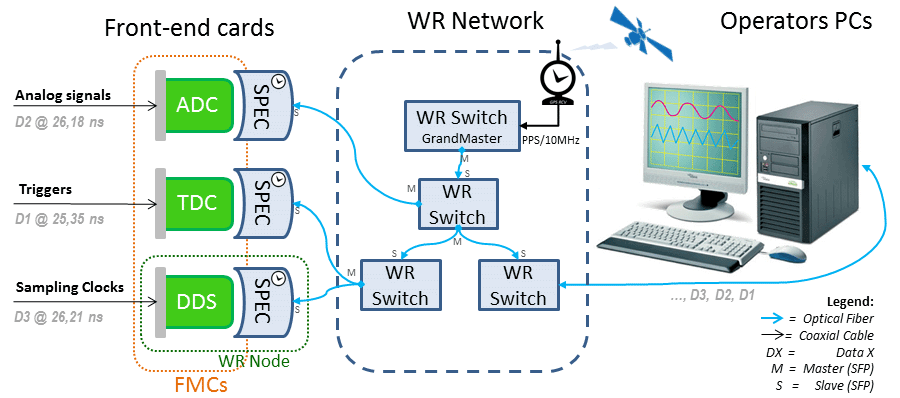
\includegraphics[width=.5\linewidth]{fig-WR-network.png}
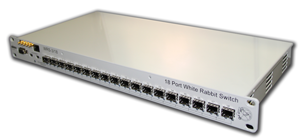
\includegraphics[width=.3\linewidth]{fig-WRS-rview.png}
\end{cdrfigure}

The WR application in $\mu$TCA standard is targeted for the moment to
easily interconnect different $\mu$TCA cards between them. The switch
can therefore be connected directly to its different nodes in the same
rack to improve maintenance and limit the space occupancy. In the
future it may be very powerful to have a full integration of the WR
within the $\mu$TCA DAQ system. For the moment the implementation
scheme in based on the integration of a WR mezzanine board on the MCH
of each shelf. This development is in progress for the WA105
demonstrator (on a MHC produced by the company NAT) with a clear
interest and collaboration by the companies producing the MCH and the
WR slave to be integrated.
